\usetikzlibrary{arrows.meta}
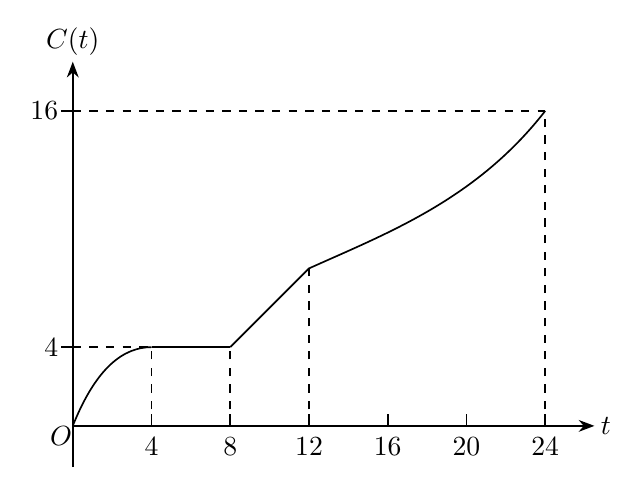
\begin{tikzpicture}[x=0.25cm,y=0.25cm,line width=.6pt,>=Stealth,font=\normalsize]
\coordinate (A0) at (0,0);
\coordinate (A4) at (4,4);
\coordinate (A8) at (8,4);
\coordinate (A12) at (12,8);
\coordinate (A16) at (16,10);
\coordinate (A20) at (20,12.6);
\coordinate (A24) at (24,16);
\draw[->] (0,0)--(26.5,0);
\node[right,inner sep=0pt,xshift=2pt] at (26.5,0) {$t$};
\draw[->] (0,-2.1)--(0,18.5);
\node[above,inner sep=0pt,yshift=2pt] at (0,18.5) {$C(t)$};
\node[below left,inner sep=0pt] at (0,0) {$O$};
\draw (4,0)--(4,0.6);
\draw (8,0)--(8,0.6);
\draw (12,0)--(12,0.6);
\draw (16,0)--(16,0.6);
\draw (20,0)--(20,0.6);
\draw (24,0)--(24,0.6);
\draw (0,4)--(-0.6,4);
\draw (0,16)--(-0.6,16);
\node[below,inner sep=0pt,yshift=-4pt] at (4,0) {$4$};
\node[below,inner sep=0pt,yshift=-4pt] at (8,0) {$8$};
\node[below,inner sep=0pt,yshift=-4pt] at (12,0) {$12$};
\node[below,inner sep=0pt,yshift=-4pt] at (16,0) {$16$};
\node[below,inner sep=0pt,yshift=-4pt] at (20,0) {$20$};
\node[below,inner sep=0pt,yshift=-4pt] at (24,0) {$24$};
\node[left,inner sep=1pt,xshift=-4pt] at (0,4) {$4$};
\node[left,inner sep=1pt,xshift=-4pt] at (0,16) {$16$};
\draw[dashed] (0,4)--(4,4);
\draw[dashed] (0,16)--(24,16);
\draw[dashed] (4,0)--(4,4);
\draw[dashed] (8,0)--(8,4);
\draw[dashed] (12,0)--(12,8);
\draw[dashed] (24,0)--(24,16);
\draw (A0) .. controls (1.2,3) and (2.6,4) .. (A4);
\draw (A4)--(A8);
\draw (A8)--(A12) .. controls (16,9.8) and (20.5,11.5) .. (A24);
\end{tikzpicture}
